\documentclass[xcolor=dvipsnames,mathserif,9pt]{beamer} %handout
%\usefonttheme{serif}%{structurebold}%{structuresmallcapsserif}%{serif}

%\input{before_document}
\usepackage{graphicx}
\usepackage{amsmath}
\usepackage{amssymb}
\usepackage[font=footnotesize]{caption} % set the captain font size to 8 (i.e. footnotesize)
\usepackage{subfig} % uses subfloats within a single float MUST after the package {caption}!!
\usepackage{natbib}
%\usepackage{cite} % sort the reference in the article by number or alphabatic
\usepackage{color}
\usepackage{algorithm} % options: boxed [section]
\usepackage{algpseudocode} % for algorithm
%\usepackage{enumerate}
\usepackage{enumitem} % directly use itemize, easily specify indent and everything
\setlist[itemize]{leftmargin=*,label=$\bullet$}%leftmargin=*,itemsep=0pt} %topsep=5pt
\setlist[enumerate]{label={\arabic*)}}
\usepackage{hyperref}
\usepackage{wrapfig}
\usepackage{textpos}
\usepackage{bibentry} % for publication list
\makeatletter\let\saved@bibitem\@bibitem\makeatother % make hyperref and bibentry compatible!!!
\nobibliography*
\usepackage{fancybox}% shadow for image
%\usepackage{empheq} % emphasize equations
\usepackage{bm}
\usepackage{arydshln} % for dashline in table or matrix
\linespread{1.3}
\usepackage{multimedia}

\usepackage{setspace} \setstretch{1.2}

\usepackage{framed}
\colorlet{shadecolor}{black!5}
% for box, page breakable, very good!!
\usepackage[framemethod=TikZ]{mdframed}%
\mdfdefinestyle{myFrame}{%
    linecolor=gray!15!white,%gray
    outerlinewidth=0.1pt,
    roundcorner=3pt,
    skipabove=15pt, % the space before the entire box
    skipbelow=15pt, % the space after the entire box. Please see the figure 2 in the manual, very clear!
    innertopmargin=10pt,%\baselineskip,
    innerbottommargin=10pt,%\baselineskip,
    %innerrightmargin=10pt,
    %innerleftmargin=10pt,
    splittopskip=\baselineskip,
    splitbottomskip=\baselineskip,
    backgroundcolor=gray!10!white,
    frametitlerule=true,
    frametitlebackgroundcolor=gray!20!white,
    frametitleaboveskip=5pt,
    frametitlebelowskip=5pt,
}
\mdfdefinestyle{myAlgo}{%
    linecolor=gray!100!white,%gray
    outerlinewidth=0.1pt,
    roundcorner=3pt,
    skipabove=15pt, % the space before the entire box
    skipbelow=15pt, % the space after the entire box. Please see the figure 2 in the manual, very clear!
    innertopmargin=10pt,%\baselineskip,
    innerbottommargin=10pt,%\baselineskip,
    %innerrightmargin=10pt,
    %innerleftmargin=10pt,
    splittopskip=\baselineskip,
    splitbottomskip=\baselineskip,
    backgroundcolor=gray!0!white,
    frametitlerule=true,
    frametitlebackgroundcolor=gray!20!white,
    frametitleaboveskip=5pt,
    frametitlebelowskip=5pt,
}


\usepackage{tikz}
\usetikzlibrary{calc} % for calculation functions in Tikz let, in commands in Tikz
\usetikzlibrary{shapes} % for block diagram
\usetikzlibrary{chains}
\usetikzlibrary{fit}
\usetikzlibrary{arrows}
\usetikzlibrary{decorations.text} % text along path

\newcommand{\blue}[1]{\textcolor{blue}{#1}}
\definecolor{myred}{RGB}{200,0,0}
\newcommand{\red}[1]{\textcolor{myred}{#1}} %magenta purple
\newcommand{\I}{\mathcal{I}}
\newcommand{\tr}{\mathrm{tr}}
\newcommand{\Null}{\mathrm{Null}}
\newcommand{\Range}{\mathrm{Range}}
\newcommand{\one}{\mathbf{1}}
\newcommand{\rank}{\mathrm{rank}}
\newcommand{\myspan}{\mathrm{span}}
\newcommand{\mydiag}{\mathrm{diag}}
\newcommand{\D}{\mathrm{d}}
\renewcommand{\d}{\mathrm{d}}
\newcommand{\blkdiag}{\mathrm{blkdiag}}
\newcommand{\sgn}{\mathrm{sgn}}
\newcommand{\T}{\mathrm{T}}
\newcommand{\myqed}{\hfill$\blacksquare$}
\newcommand{\ep}{\varepsilon}
\newcommand{\sig}{\mathrm{sig}_a}
%\newcommand{\sigep_}[1]{\sig(\ep_{#1})}
\newcommand{\R}{\mathbb{R}}
\newcommand{\A}{\mathcal{A}}
\newcommand{\G}{\mathcal{G}}
\newcommand{\E}{\mathbb{E}}
\newcommand{\X}{\mathcal{X}}
\newcommand{\V}{\mathcal{V}}
\newcommand{\N}{\mathcal{N}}
\newcommand{\M}{\mathcal{M}}
\renewcommand{\H}{\mathcal{H}}
\renewcommand{\L}{\mathcal{B}}
\renewcommand{\S}{\mathcal{S}}
\newcommand{\xe}{x_{\text{e}}}
%\newcommand{\Null}[1]{\mathrm{Null}\left(#1\right)}
\newcommand{\sk}[1]{\left[#1\right]_\times} % skew symmetric operator
\newcommand{\dia}[1]{\mathrm{diag}\left(#1\right)} % block diagnal matrix
%\renewcommand{\span}[1]{\mathrm{span}\left\{#1\right\}} % ERROR when redefine \span
\newcommand{\Var}{\mathrm{Var}}
\newcommand{\var}{\mathrm{var}}


\graphicspath{{figures/}}

% for tikz, theorem, lemma ... environments have already been declared. You don't need to declare, or you need to use other names than theorem or lemma, such as my_theorem.
%\newtheorem{my_theorem}{Theorem}
%\newtheorem{my_lemma}{Lemma}
\newtheorem{assumption}{Assumption} % necessary for beamer
%\newtheorem{my_remark}{Remark}
\newtheorem{proposition}{Proposition} % necessary for beamer
%\newtheorem{my_corollary}{Corollary}
%\newtheorem{my_example}{Example}
%\newtheorem{my_definition}{Definition}
%\newtheorem{my_problem}{Problem}

%##################################################
\newcommand{\pagetitle}[1]{\textbf{\textcolor{BlueViolet}{$\circ$ #1}}} %!!!
\newcommand{\pagehighlight}[1]{\textbf{\textcolor{Brown}{#1}}} %!!!
\newcommand{\mypause}{\pause} % this is useful for slide show. if you don't want pause any more, just set it as blank
%\newcommand{\mybullet}{\textcolor{BlueViolet}{$\blacksquare$} }%{$\rhd$ }
%\newcommand{\myhighsign}{$\star$ }% the sign to highlight a sentence

%##################################################
% To highlight equation. Example: \begin{align*} \boxed{xxx} \end{align*}
% does not support multiline equations
% put color to \boxed math command
\newcommand*{\boxcolor}{gray}
\makeatletter
\renewcommand{\boxed}[1]{\textcolor{\boxcolor}{%
%\tikz[baseline={([yshift=-1ex]current bounding box.center)}] \node [rectangle, minimum width=1ex,rounded corners,draw] {\normalcolor\m@th$\displaystyle#1$};}}
\tikz[baseline={([yshift=-1ex]current bounding box.center)}] \node [rectangle, minimum width=2ex,rounded corners,draw] {\normalcolor\m@th$\displaystyle#1$};}}
\makeatother

%##################################################
% set my own theme
\def\structureHeight{9mm}
\usetheme[height=\structureHeight]{Rochester}
\usecolortheme[RGB={0,0,128}]{structure}
\setbeamertemplate{items}[circle]%rectangle, triangle,circle
\setbeamertemplate{blocks}[rounded][shadow=true]
\setbeamertemplate{navigation symbols}{}
%\addtobeamertemplate{frametitle}{} % specify the logo
%{
%    \begin{textblock*}{100mm}(.87\textwidth,-\structureHeight)
%        \includegraphics[height=6.6mm,width=3cm,keepaspectratio]{../common_figures_private/westlake_logo.png} % add logo
%    \end{textblock*}
%}
\addtobeamertemplate{frametitle}{\vskip4pt}{} % specify
%\setbeamerfont{frametitle}{size=\large}
\definecolor{mylightgray}{RGB}{240 240 240}
\definecolor{mykhaki}{RGB}{240 230 140}% khaki color
\definecolor{mylightYellow}{RGB}{255,255,224} % light yellow
%\setbeamercolor{beamercolor1}{bg=mylightgray, fg=black}
%\setbeamercolor{beamercolor2}{bg=mylightYellow,fg=black}%{bg=yellow!90!white, fg=black}
% background and foreground color
\setbeamercolor{background canvas}{bg=black!0!white} % background color of every slide! My previous value was black!10!white for my lecture videos!
\setbeamercolor{normal text}{bg=black!10!white} % background color for e.g. theorem environment. When canvas is 10, here it can be 20; the bg for normal text changes the color of hidden text when you use overlay

\setbeamercolor{block title}{bg=mykhaki,fg=black}
\defbeamertemplate{footline}{zsy_frameNumber}
{%
  \hspace{5pt}  \emph{Shiyu Zhao}
  \hspace*{\fill}%
  \usebeamercolor[fg]{page number in head/foot}%
  \insertframenumber\,/\,\inserttotalframenumber \vspace{0pt} \hspace{5pt}
  \vskip5pt
}
\setbeamertemplate{footline}[zsy_frameNumber]
%##################################################
\setbeamercovered{transparent=0} % a good value for transparent text is 20
% when using the overlay commands like \onslide or \uncover, the text will NOT be invisible, instead it will be like transparent
%\pause will also have the transparent effect: command \pause is easy to use: to make it invisible, change the value to zero.



\usepackage{multimedia}
\linespread{1.3}
\newcommand{\hl}{$\triangleright$ }
%\newcommand{\blue}[1]{\textcolor{blue}{#1}}
%\newcommand{\red}[1]{\textcolor{red}{#1}}

\begin{document}

%%%%%%%%%%%%%%%%%%%%%%%%%%%%%%%%%%%%%%%%%%%%%%%%%%%%%%%%%%%%%%%%%%%%%%%%%%%%%%%%%
% define the author, date etc. information
%\subtitle{Mathematical and Biological Foundation for Reinforcement Learning}
\title{Lecture 2: State Value and Bellman Equation}

\author{Shiyu Zhao
\newline
\newline {\small Department of Artificial Intelligence}
\newline {\small Westlake University}
}
%\logo{\includegraphics[width=1cm,height=1cm,keepaspectratio]{NUSLogo.png}~}
%\date{\today}
\date{}
\subject{}


%%%%%%%%%%%%%%%%%%%%%%%%%%%%%%%%%%%%%%%%%%%%%%%%%%%%%%%%%%%%%%%%%%%%%%%%%%%%%%%%%

{
\setbeamertemplate{footline}{} % remove the frame number of the title page
\begin{frame}
    %\frametitle{Lecture: Networked Dynamic Systems}
    \addtocounter{framenumber}{-1} % discounter the title page, otherwise the frame number starts from 2 instead of 1
    \titlepage % this only gives the author etc. information
\end{frame}
}


%------------------------------------------
\begin{frame}
\frametitle{Outline}
\begin{figure}[h]
  \centering
\includegraphics[width=0.8\linewidth]{Figure_chapterRelationship.pdf}
\end{figure}
\end{frame}
%------------------------------------------
\begin{frame}
\frametitle{Outline}
In this lecture:
\begin{itemize}
\item Core concepts: optimal state value and optimal policy
\item A fundamental tool: Bellman optimality equation (BOE)
\end{itemize}

\end{frame}
%%******************************************************************************
\begin{frame}
\frametitle{Outline}
\tableofcontents
\end{frame}
\AtBeginSection[]% put it to the start of each section
{
  \begin{frame}
    \frametitle{Outline}
    \tableofcontents[currentsection]
  \end{frame}
}%
%%******************************************************************************
%\AtBeginSection[]% put it to the start of each section
%{
%  \begin{frame}
%    \frametitle{Outline}
%    \tableofcontents[currentsection]
%  \end{frame}
%}
%\section{Revisit the last lecture}
%%------------------------------------------------------
%\begin{frame}
%\frametitle{Revisit the last lecture}
%
% State value:
%$$v_\pi(s)=\E[G_{t}|S_t=s]$$
%
%\pause
% The Bellman equation (elementwise form):
%\begin{align*}
%\textcolor{red}{v_\pi(s)}
%&=\textcolor{black}{\sum_{a}\pi(a|s)\Big[\underbrace{\sum_{r}p(r|s,a)r}_{\substack{\text{immediate reward}\\ \text{after taking action $a$}}}+\underbrace{\gamma \sum_{s'} p(s'|s,a)\textcolor{red}{v_\pi(s')}}_{\substack{\text{discounted future reward}\\ \text{after taking action $a$}}}\Big]}
%\end{align*}
%
%\end{frame}
%%----------------------------------------------------
%\begin{frame}
%\frametitle{Revisit the last lecture}
%
% The Bellman equation (matrix-vector form):
%\begin{align*}
%\textcolor{blue}{v_\pi=r_\pi+\gamma  P_\pi v_\pi},
%\end{align*}
%\pause
%where
%\begin{align*}
%v_\pi=\left[
%  \begin{array}{c}
%     v_\pi(s_1)\\
%     \vdots\\
%     v_\pi(s_n)\\
%  \end{array}
%\right]\in\R^{n},\quad
%r_\pi=\left[
%  \begin{array}{c}
%     r_\pi(s_1)\\
%     \vdots\\
%     r_\pi(s_n)\\
%  \end{array}
%\right]\in\R^{n},\quad
%[P_\pi]_{ij}=p_\pi(s_j|s_i)
%\end{align*}
%and
%\begin{align*}
%v_\pi(s_i)=r_\pi(s_i)+\gamma  \sum_{s_j}p_\pi(s_j|s_i)v_\pi(s_j)
%\end{align*}
%\end{frame}
%%----------------------------------------------------
%\begin{frame}
%\frametitle{Revisit the last lecture}
%
% Action value:
%
%$$q_{\pi}(s,a):=\E[G_t|S_t=s,A_t=a]$$
%
%\pause
%Calculate action value from state value:
%\begin{align*}
%\textcolor{red}{q_\pi(s,a)}
%&=\sum_{r}p(r|s,a)r+\gamma  \sum_{s'} p(s'|s,a)\textcolor{red}{v_\pi(s')}
%\end{align*}
%
%\pause
%Calculate state value from action value:
%\begin{align*}%\label{eq_statevalueandactionvalue}
%\textcolor{black}{v_{\pi}(s)=\sum_a \pi(a|s)q_{\pi}(s,a)}
%\end{align*}
%\end{frame}
%%******************************************************************************
%\begin{frame}
%\frametitle{Revisit the last lecture - Example}
%\begin{figure}[h]
%  \centering
%  \includegraphics[width=0.2\linewidth]{fig_Bellman_demoReturnPolicy2}
%\end{figure}
% Bellman equation:
%\begin{align*}
%v_{\pi}(s_1)&=-1+\gamma v_{\pi}(s_2),\\
%v_{\pi}(s_2)&=+1+\gamma v_{\pi}(s_4),\\
%v_{\pi}(s_3)&=+1+\gamma v_{\pi}(s_4),\\
%v_{\pi}(s_4)&=+1+\gamma v_{\pi}(s_4).
%\end{align*}
% State value: Let $\gamma=0.9$. Then, it can be calculated that
%\begin{align*}
%v_{\pi}(s_4)=v_{\pi}(s_3)=v_{\pi}(s_2)=10,\quad v_{\pi}(s_1)=8.
%\end{align*}
%\end{frame}
%%******************************************************************************
%\begin{frame}
%\frametitle{Revisit the last lecture - Example}
%\vspace{-5pt}
%\begin{figure}[h]
%  \centering
%  \includegraphics[width=0.25\linewidth]{fig_Bellman_demoReturnPolicy2}
%\end{figure}
%
% Action value: $\gamma=0.9$
%\begin{align*}
%q_\pi(s_1,a_1)&=-1+\gamma v_{\pi}(s_1)=6.2,\\
%q_\pi(s_1,a_2)&=-1+\gamma v_{\pi}(s_2)=8,\\
%q_\pi(s_1,\textcolor{blue}{a_3})&=0+\gamma v_{\pi}(s_3)=9,\\
%q_\pi(s_1,a_4)&=-1+\gamma v_{\pi}(s_1)=6.2,\\
%q_\pi(s_1,a_5)&=0+\gamma v_{\pi}(s_1)=7.2.
%\end{align*}
%\end{frame}
%******************************************************************************
\AtBeginSection[]% put it to the start of each section
{
  \begin{frame}
    \frametitle{Outline}
    \tableofcontents[currentsection]
  \end{frame}
}
\section{Motivating examples}
%******************************************************************************
\begin{frame}
\frametitle{Motivating examples}
\begin{figure}[h]
  \centering
  \includegraphics[width=0.25\linewidth]{fig_Bellman_demoReturnPolicy2}
\end{figure}
\textbf{Exercise:} write out the Bellman equation and solve the state values (set $\gamma=0.9$)

\pause
\textbf{Answer: }Bellman equations:
\begin{align*}
v_{\pi}(s_1)&=-1+\gamma v_{\pi}(s_2),\\
v_{\pi}(s_2)&=+1+\gamma v_{\pi}(s_4),\\
v_{\pi}(s_3)&=+1+\gamma v_{\pi}(s_4),\\
v_{\pi}(s_4)&=+1+\gamma v_{\pi}(s_4).
\end{align*}
State values: $v_{\pi}(s_4)=v_{\pi}(s_3)=v_{\pi}(s_2)=10,v_{\pi}(s_1)=8$
\end{frame}
%-----------------------------------
\begin{frame}
\frametitle{Motivating examples}
\vspace{-5pt}
\begin{figure}[h]
  \centering
  \includegraphics[width=0.25\linewidth]{fig_Bellman_demoReturnPolicy2}
\end{figure}

\textbf{Exercise:} calculate the action values of the five actions for $s_1$

\pause
\textbf{Answer:}
Action values:
\begin{align*}
q_\pi(s_1,a_1)&=-1+\gamma v_{\pi}(s_1)=6.2,\\
q_\pi(s_1,a_2)&=-1+\gamma v_{\pi}(s_2)=8,\\
q_\pi(s_1,\textcolor{blue}{a_3})&=0+\gamma v_{\pi}(s_3)=9,\\
q_\pi(s_1,a_4)&=-1+\gamma v_{\pi}(s_1)=6.2,\\
q_\pi(s_1,a_5)&=0+\gamma v_{\pi}(s_1)=7.2.
\end{align*}
\end{frame}
%------------------------------------------
\begin{frame}
\frametitle{Motivating examples}
\begin{figure}[h]
  \centering
  \includegraphics[width=0.25\linewidth]{fig_Bellman_demoReturnPolicy2}
  %\includegraphics[width=0.25\linewidth]{fig_Bellman_demoReturnPolicy1}
\end{figure}

\textbf{Question:} While the policy is not good, how can we improve it?
\pause

\textbf{Answer:} We can improve the policy based on action values.

In particular, the current policy $\pi(a|s_1)$ is
\begin{align*}
\pi(a|s_1)=
\left\{
  \begin{array}{ll}
   1 & a=a_2 \\
   0 & a\ne a_2 \\
  \end{array}
\right.
\end{align*}

\end{frame}
%******************************************************************************
\begin{frame}
\frametitle{Motivating examples}
\begin{figure}[h]
  \centering
  \includegraphics[width=0.2\linewidth]{fig_Bellman_demoReturnPolicy2}
\end{figure}
 Observe the action values that we obtained just now:
\begin{align*}
&q_\pi(s_1,a_1)=6.2, \quad q_\pi(s_1,a_2)=8, \quad q_\pi(s_1,\blue{a_3})=9, \\
&q_\pi(s_1,a_4)=6.2, \quad q_\pi(s_1,a_5)=7.2.
\end{align*}

\pause
 What if we select the \blue{greatest action value}? Then, the \blue{new policy} is
\begin{align*}
\pi_{\text{new}}(a|s_1)=
\left\{
  \begin{array}{ll}
   1 & a=a_3 \\
   0 & a\ne a_3 \\
  \end{array}
\right.
\end{align*}
The new policy can avoid the forbidden area and seems better.
\end{frame}
%******************************************************************************
\begin{frame}
\frametitle{Motivating examples}
\begin{figure}[h]
  \centering
  \includegraphics[width=0.25\linewidth]{fig_Bellman_demoReturnPolicy2}
\end{figure}

 \textcolor{blue}{Question: why doing this can improve the policy?}

\begin{itemize}
\item Intuition: easy! Actions with greater values are better.
\item Math: nontrivial! Will be introduced in this and next lectures!
\end{itemize}

\end{frame}
%******************************************************************************
\AtBeginSection[]% put it to the start of each section
{
  \begin{frame}
    \frametitle{Outline}
    \tableofcontents[currentsection]
  \end{frame}
}
\section{Definition of optimal policy}

%----------------------------------------------------
\begin{frame}
\frametitle{Optimal policy}

State value can be used to evaluate whether a policy is good or not: if
$$v_{\pi_1}(s)\ge v_{\pi_2}(s) \quad \text{for all } s\in\S$$
then $\pi_1$ is \blue{better} than $\pi_2$.

\pause
\begin{definition}
Policy $\pi^*$ is optimal if $v_{\pi^*}(s)\ge v_{\pi}(s)$ for any other policy $\pi$ and for all $s\in\S$.
\end{definition}

\pause
The definition leads to many \textbf{questions}:
\begin{itemize}
\item Does the optimal policy exist?
\item Is the optimal policy unique?
\item Is the optimal policy stochastic or deterministic?
\item How to obtain the optimal policy?
\end{itemize}
\pause
 To answer these questions, we need the \blue{Bellman optimality equation}.

\end{frame}
%******************************************************************************
\AtBeginSection[]% put it to the start of each section
{
  \begin{frame}
    \frametitle{Outline}
    \tableofcontents[currentsection]
  \end{frame}
}
\section{BOE: Introduction}
%----------------------------------------------------
\begin{frame}
\frametitle{Bellman optimality equation (BOE)}

 \textbf{Bellman optimality equation (elementwise form):}
\begin{align*}
v(s)
&=\visible<2->{\blue{\max_\pi}} \sum_{a}\blue{\pi(a|s)}\left(\sum_{r}p(r|s,a)r + \gamma \sum_{s'}p(s'|s,a)v(s')\right),\quad s\in\mathcal{S}\\
\visible<3->{&=\blue{\max_\pi} \sum_{a}\blue{\pi(a|s)} q(s,a),\quad s\in\S}
\end{align*}

\visible<4->{
Remarks:
\begin{itemize}
\item $p(r|s,a), p(s'|s,a)$, $r$, $\gamma$ are \blue{known}.
\item $v(s),v(s')$ are \blue{unknown} and to be calculated.
\item Is $\pi(s)$ known or unknown? \blue{It is unknown and to be calculated!}
\end{itemize}
}
\end{frame}
%----------------------------------------------------
\begin{frame}
\frametitle{Bellman optimality equation (BOE)}

 \textbf{Bellman optimality equation (matrix-vector form):}
\begin{align*}%\label{eq_bellmanOptimalityEquation_matrixForm}
\red{v=\max_{\pi}(r_\pi+\gamma  P_\pi v)}
\end{align*}
where the elements corresponding to $s$ or $s'$ are
\begin{align*}
&[r_\pi]_s\triangleq\sum_{a}\pi(a|s)\sum_{r}p(r|s,a)r,\\ &[P_{\pi}]_{s,s'}=p(s'|s)\triangleq\sum_{a}\pi(a|s)\sum_{s'}p(s'|s,a)
\end{align*}
Here $\max_\pi$ is performed elementwise:
\begin{align*}
\max_\pi\left[
  \begin{array}{c}
    * \\
    \vdots \\
    * \\
  \end{array}
\right]
=
\left[
  \begin{array}{c}
    \max_{\pi(s_1)}* \\
    \vdots \\
    \max_{\pi(s_n)}* \\
  \end{array}
\right]
\end{align*}

\end{frame}
%----------------------------------------------------
\begin{frame}
\frametitle{Bellman optimality equation (BOE)}

 \textbf{Bellman optimality equation (matrix-vector form):}
\begin{align*}%\label{eq_bellmanOptimalityEquation_matrixForm}
\red{v=\max_{\pi}(r_\pi+\gamma  P_\pi v)}
\end{align*}

\begin{itemize}
\item BOE is \blue{tricky} yet \blue{elegant}!
\begin{itemize}
\item[-] Why elegant? It describes the optimal policy and optimal state value in an elegant way.
\item[-] Why tricky? There is a maximization on the right-hand side, which may not be straightforward to see how to compute.
\end{itemize}
\pause
\item This lecture will answer all the following questions:
\begin{itemize}
\item[-] \textbf{Algorithm}: how to solve this equation?
\item[-] \textbf{Existence}: does this equation have solutions?
\item[-] \textbf{Uniqueness}: is the solution to this equation unique?
\item[-] \textbf{Optimality}: how is it related to optimal policy?
\end{itemize}
\end{itemize}
\end{frame}
%******************************************************************************
\AtBeginSection[]% put it to the start of each section
{
  \begin{frame}
    \frametitle{Outline}
    \tableofcontents[currentsection]
  \end{frame}
}
\section{BOE: Preliminaries}
%******************************************************************************
\AtBeginSubsection[]% note: it is AtBeginSubsection here! subsection
{
  \begin{frame}
    \frametitle{Outline}
    \tableofcontents[currentsection,currentsubsection]
  \end{frame}
}
\subsection{BOE: Maximization on the right-hand side}
%----------------------------------------------------
\begin{frame}
\frametitle{Maximization on the right-hand side of BOE}
 BOE: elementwise form
\begin{align*}
v(s)
&={\blue{\max_\pi}} \sum_{a}\blue{\pi(a|s)}\left(\sum_{r}p(r|s,a)r + \gamma \sum_{s'}p(s'|s,a)v(s')\right),\quad \forall s\in\mathcal{S}
%\visible<3->{&=\blue{\max_\pi} \sum_{a}\blue{\pi(a|s)} q(s,a)}\quad s\in\S
\end{align*}
 BOE: matrix-vector form
\begin{align*}%\label{eq_bellmanOptimalityEquation_matrixForm}
\red{v=\max_{\pi}(r_\pi+\gamma  P_\pi v)}
\end{align*}

\pause
\begin{example}[How to solve two unknowns from one equation]%\label{example_solveTwoUnknownsFromOneEq}
Solve two unknown variables $x,a\in\R$ from the following equation:
$$x=\max_a (2x-1-a^2).$$
To solve them, first consider the right hand side. Regardless the value of $x$, $\max_a (2x-1-a^2)=2x-1$ where the maximization is achieved when $a=0$. Second, when $a=0$, the equation becomes $x=2x-1$, which leads to $x=1$. Therefore, $a=0$ and $x=1$ are the solution of the equation.
\end{example}

\end{frame}
%----------------------------------------------------
\begin{frame}
\frametitle{Maximization on the right-hand side of BOE}
\vspace{-5pt}
 Fix $v'(s)$ first and solve $\pi$:
\begin{align*}
v(s)
&=\blue{\max_\pi} \sum_{a}\blue{\pi(a|s)}\left(\sum_{r}p(r|s,a)r + \gamma \sum_{s'}p(s'|s,a)v(s')\right),\quad \forall s\in\mathcal{S}\\
&=\blue{\max_\pi} \sum_{a}\blue{\pi(a|s)} q(s,a)
\onslide<2->{=\blue{\max_\pi} \left[\blue{\pi(a_1|s)} q(s,a_1)+\dots+\blue{\pi(a_5|s)} q(s,a_5)\right]\\}
&\onslide<5->{\doteq\blue{\max_{c_1,\dots,c_5}} \left[\blue{c_1} q(s,a_1)+\dots+\blue{c_5} q(s,a_5)\right],\qquad c_1+\dots+c_5=1}
\end{align*}

\onslide<3->{
\begin{example}[How to solve ${\max_\pi} \sum_{a}{\pi(a|s)} q(s,a)$]%\label{example_solveTwoUnknownsFromOneEq}
Suppose $q_1,q_2,q_3\in\R$ are given. Find $c_1^*,c_2^*,c_3^*$ solving
\vspace{-5pt}
\begin{align*}
\max_{c_1,c_2,c_3} c_1q_1+c_2q_2+c_3q_3
\end{align*}
where $c_1+c_2+c_3=1$ and $c_1,c_2,c_3\ge0$.

\onslide<4->{
Answer: Suppose $q_3\ge q_1,q_2$. Then, the optimal solution is $c_3^*=1$ and $c_1^*=c_2^*=0$. That is because for any $c_1,c_2,c_3$
\vspace{-10pt}
$$q_3=(c_1+c_2+c_3)q_3=c_1q_3+c_2q_3+c_3q_3\ge c_1q_1+c_2q_2+c_3q_3$$
}
\vspace{-15pt}
\end{example}}

\end{frame}
%----------------------------------------------------
\begin{frame}
\frametitle{Maximization on the right-hand side of BOE}
Inspired by the above example, considering that $\sum_a \pi(a|s)=1$, we have
\begin{align*}
v(s)
&=\blue{\max_\pi} \sum_{a}\blue{\pi(a|s)}\left(\sum_{r}p(r|s,a)r + \gamma \sum_{s'}p(s'|s,a)v(s')\right),\quad \forall s\in\mathcal{S}\\
&=\blue{\max_\pi} \sum_{a}\blue{\pi(a|s)} q(s,a)\\
&=\red{\max_{a\in\A(s)} q(s,a)}
\end{align*}
where the optimality is achieved when
\begin{align*}
\pi(a|s)=
\left\{
  \begin{array}{ll}
   1 & a=a^* \\
   0 & a\ne a^* \\
  \end{array}
\right.
\end{align*}
where $a^*=\arg\max_a q(s,a)$.

\end{frame}
%******************************************************************************
\AtBeginSubsection[]% note: it is AtBeginSubsection here! subsection
{
  \begin{frame}
    \frametitle{Outline}
    \tableofcontents[currentsection,currentsubsection]
  \end{frame}
}
\subsection{BOE: Rewrite as $v=f(v)$}
%----------------------------------------------------
\begin{frame}
\frametitle{Solve the Bellman optimality equation}

 The BOE is $v=\max_\pi (r_\pi+\gamma P_{\pi}v)$. \pause Let
$$f(v):=\max_\pi (r_\pi+\gamma P_{\pi}v)$$

\pause
Then, the Bellman optimality equation becomes
$$v=f(v)$$
where
\begin{align*}
[f(v)]_{s}=\max_\pi \sum_{a}\pi(a|s)q(s,a), \quad s\in\S
\end{align*}
\blue{This equation looks very simple. How to solve it?}
\end{frame}
%******************************************************************************
\AtBeginSubsection[]% note: it is AtBeginSubsection here! subsection
{
  \begin{frame}
    \frametitle{Outline}
    \tableofcontents[currentsection,currentsubsection]
  \end{frame}
}
\subsection{Contraction mapping theorem}
%----------------------------------------------------
\begin{frame}
\frametitle{Preliminaries: Contraction mapping theorem}

 Some concepts:
\begin{itemize}
\item \blue{Fixed point:} $x\in X$ is a fixed point of $f: X\rightarrow X$ if $$f(x)=x$$
\vspace{-10pt}
\pause
\item \blue{Contraction mapping (or contractive function):} $f$ is a contraction mapping if $$\|f(x_1)-f(x_2)\|\le \gamma  \|x_1-x_2\|$$
    where $\gamma \in(0,1)$.
\begin{itemize}
\item[-] $\gamma $ must be strictly less than $1$ so that many limits such as $\gamma^k\rightarrow0$ as $k\rightarrow0$ hold.
\item[-] Here $\|\cdot\|$ can be any vector norm.
\end{itemize}
\end{itemize}

\end{frame}
%----------------------------------------------------
\begin{frame}
\frametitle{Preliminaries: Contraction mapping theorem}
Examples to demonstrate the concepts.
\begin{example}
\begin{itemize}
\item $x=f(x)=0.5x$, $x\in\R$.

It is easy to verify that $x=0$ is a fixed point since $0=0.5\times 0$. Moreover, $f(x)=0.5x$ is a contraction mapping because $\|0.5x_1-0.5x_2\|=0.5\|x_1-x_2\|\le \gamma \|x_1-x_2\|$ for any $\gamma\in[0.5,1)$.
\end{itemize}
\pause
\begin{itemize}
\item $x=f(x)=Ax$, where $x\in\R^n, A\in\R^{n\times n}$ and $\|A\|\le\gamma<1$.

It is easy to verify that $x=0$ is a fixed point since $0=A0$. To see the contraction property, $\|Ax_1-Ax_2\|=\|A(x_1-x_2)\|\le \|A\|\|x_1-x_2\|\le\gamma\|x_1-x_2\|$. Therefore, $f(x)=Ax$ is a contraction mapping.
\end{itemize}
\end{example}

\end{frame}%
%%----------------------------------------------------
%\begin{frame}
%\frametitle{Preliminaries: Contraction mapping theorem}
%Examples to demonstrate the concepts.
%\begin{example}
%\begin{itemize}
%\item $x=f(x)=0.5\sin x$, $x\in\R$.
%
%It is easy to see that $x=0$ is a fixed point since $0=0.5\sin0$. Moreover, it follows from the \emph{mean value theorem} that
%\begin{align*}
%\left|\frac{0.5\sin x_1-0.5\sin x_2}{x_1-x_2}\right|=|0.5\cos x_3|\le 0.5, \quad x_3\in(x_1,x_2).
%\end{align*}
%Hence, $|0.5\sin x_1-0.5\sin x_2|\le 0.5 |x_1-x_2|$ and $f(x)=0.5\sin x$ is a contraction mapping.
%\end{itemize}
%\end{example}
%
%\end{frame}
%----------------------------------------------------
\begin{frame}
\frametitle{Preliminaries: Contraction mapping theorem}

\begin{theorem}[{Contraction Mapping Theorem}]
For any equation that has the form of $x=f(x)$, if $f$ is a contraction mapping, then
\begin{itemize}
\item \textbf{Existence}: there exists a fixed point $x^*$ satisfying $f(x^*)=x^*$.
\item \textbf{Uniqueness}: The fixed point $x^*$ is unique.
\item \textbf{Algorithm}: Consider a sequence $\{x_k\}$ generated by 
$$x_{k+1}=f(x_k)$$
then $x_k\rightarrow x^*$ as $k\rightarrow\infty$. Moreover, the convergence rate is \emph{exponentially fast}.
\end{itemize}
\end{theorem}

For the proof of this theorem, see the book.

\end{frame}
%----------------------------------------------------
\begin{frame}
\frametitle{Preliminaries: Contraction mapping theorem}

 Examples:

\begin{itemize}
\item $x=0.5x$, where $f(x)=0.5x$ and $x\in\R$

$x^*=0$ is the unique fixed point. It can be solved iteratively by
$$x_{k+1}=0.5x_k$$
\pause
\item $x=Ax$, where $f(x)=Ax$ and $x\in\R^n, A\in\R^{n\times n}$ and $\|A\|<1$

$x^*=0$ is the unique fixed point. It can be solved iteratively by
$$x_{k+1}=Ax_k$$

%\item $x=0.5\sin x$, where $f(x)=0.5\sin x$ and $x\in\R$.
%
%$x^*=0$ is the unique fixed point. It can be solved iteratively by
%$$x_{k+1}=0.5 \sin x_k$$
\end{itemize}
\end{frame}
%******************************************************************************
\AtBeginSection[]% put it to the start of each section
{
  \begin{frame}
    \frametitle{Outline}
    \tableofcontents[currentsection]
  \end{frame}
}
\section{BOE: Solution}
%----------------------------------------------------
\begin{frame}
\frametitle{Contraction property of BOE}

Let's come back to the Bellman optimality equation:
$$v=f(v)=\max_\pi (r_\pi+\gamma P_{\pi} v)$$

\pause
\begin{theorem}[Contraction Property]
$f(v)$ is a contraction mapping that satisfies
$$\|f(v_1)-f(v_2)\|\le\red{\gamma } \|v_1-v_2\|$$
where $\gamma$ is the discount rate!
\end{theorem}

The proof is omitted here and can be found in my book.

\end{frame}
%----------------------------------------------------
\begin{frame}
\frametitle{Solve the Bellman optimality equation}

Applying the contraction mapping theorem gives the following results.
\vspace{10pt}
\begin{theorem}[Existence, Uniqueness, and Algorithm]
For the BOE $v=f(v)=\max_\pi(r_\pi+\gamma  P_\pi v)$, there always \blue{exists} a solution $v^*$ and the solution is \blue{unique}. The solution could be solved iteratively by
\begin{align}\label{eq_algorithmBOE}
\blue{v_{k+1}= f(v_k)=\max_\pi(r_\pi+\gamma  P_\pi v_k)}
\end{align}
This sequence $\{v_k\}$ converges to $v^*$ \blue{exponentially fast} given any initial guess $v_0$. The convergence rate is parameterized by $\gamma $.
\end{theorem}
\vspace{10pt}
\pause
\textbf{Important:} The algorithm in \eqref{eq_algorithmBOE} is called the \red{value iteration algorithm}. We will analyze it in the next lecture! This lecture focuses more on the fundamental properties.

\end{frame}%
%%--------------------------------------
%\begin{frame}
%\frametitle{Solve the Bellman optimality equation}
%
% The iterative algorithm:
%
%Matrix-vector form:
%$$v_{k+1}= f(v_k)=\max_\pi(r_\pi+\gamma  P_\pi v_k)$$
%\pause
%Elementwise form:
%\begin{align*}
%\red{v_{k+1}(s)}
%&=\max_\pi \sum_{a}\blue{\pi(a|s)}{\left(\sum_{r}p(r|s,a)r + \gamma \sum_{s'}p(s'|s,a)\red{v_k(s')}\right)}\\
%&=\max_\pi \sum_{a}\blue{\pi(a|s)} q_k(s,a)\\
%&=\max_a q_k(s,a)
%\end{align*}
%\end{frame}
%%--------------------------------------
%\begin{frame}
%\frametitle{Solve the Bellman optimality equation}
% Procedure summary:
%
%\begin{itemize}
%\item For any $s$, current estimated value $v_k(s)$
%\pause
%\item For any $a\in\A(s)$, calculate $q_k(s,a)=\sum_{r}p(r|s,a)r + \gamma \sum_{s'}p(s'|s,a)v_k(s')$
%\pause
%\item Calculate the greedy policy $\pi_{k+1}$ for $s$ as
%\begin{align*}%\label{eq_existGreedyOptimalPolicyDeterministic}
%{\pi_{k+1}(a|s)=
%\left\{
%  \begin{array}{ll}
%   1 & a=a^*_k(s) \\
%   0 & a\ne a^*_k(s) \\
%  \end{array}
%\right.}
%\end{align*}
%where $a^*_{k}(s)=\arg\max_a q_{k}(s,a)$.
%\pause
%\item Calculate $v_{k+1}(s)=\max_a q_k(s,a)$
%\end{itemize}
%\pause
%The above algorithm is actually the \blue{value iteration algorithm} as discussed in the next lecture.
%\end{frame}
%******************************************************************************
\AtBeginSection[]% put it to the start of each section
{
  \begin{frame}
    \frametitle{Outline}
    \tableofcontents[currentsection]
  \end{frame}
}
\section{BOE: Optimality}
%----------------------------------------------------
\begin{frame}
\frametitle{Policy optimality}
Suppose $v^*$ is the solution to the Bellman optimality equation. It satisfies
$$v^*=\max_\pi (r_\pi+\gamma P_{\pi}v^*)$$
\pause
Suppose
$$\pi^*=\arg\max_\pi (r_\pi+\gamma P_{\pi}v^*)$$
\pause
Then
$$v^*=r_{\pi^*}+\gamma P_{\pi^*}v^*$$
Therefore, $\pi^*$ is a policy and $v^*=v_{\pi^*}$ is the corresponding state value.

\pause
\vspace{10pt}
\blue{ Is $\pi^*$ the optimal policy? Is $v^*$ the greatest state value can be achieved?}
\end{frame}
%----------------------------------------------------
\begin{frame}
\frametitle{Policy optimality}

\begin{theorem}[Policy Optimality]
Suppose that $v^*$ is the unique solution to $v=\max_{\pi}(r_\pi+\gamma  P_\pi v)$, and $v_\pi$ is the state value function satisfying $v_\pi=r_\pi+\gamma  P_\pi v_\pi$ for any given policy $\pi$, then
$$v^*\ge v_\pi,\quad \forall \pi$$
\end{theorem}
For the proof, please see my book.

\pause
\vspace{10pt}
\blue{Now we understand why we study the BOE. That is because it describes the \textbf{optimal state value} and \textbf{optimal policy}.}

\end{frame}

%----------------------------------------------------
\begin{frame}
\frametitle{Optimal policy}

What does an optimal policy $\pi^*$ look like?

$$\red{\pi^*(s)}=\arg\max_\pi \sum_{a}{\pi(a|s)}\underbrace{\left(\sum_{r}p(r|s,a)r + \gamma \sum_{s'}p(s'|s,a)\blue{v^*(s')}\right)}_{\blue{q^*(s,a)}}$$

\pause
\begin{theorem}[Greedy Optimal Policy]\label{theorem_existGreedyOptimalPolicy}
For any $s\in\S$, the deterministic greedy policy
\begin{align*}%\label{eq_existGreedyOptimalPolicyDeterministic}
{\pi^*(a|s)=
\left\{
  \begin{array}{ll}
   1 & a=a^*(s) \\
   0 & a\ne a^*(s) \\
  \end{array}
\right.}
\end{align*}
is an optimal policy solving the BOE. Here,
$$a^*(s)=\arg\max_a q^*(a,s),$$
where $q^*(s,a)\doteq\sum_{r}p(r|s,a)r + \gamma \sum_{s'}p(s'|s,a)v^*(s')$.
\end{theorem}
\end{frame}
%******************************************************************************
\AtBeginSection[]% put it to the start of each section
{
  \begin{frame}
    \frametitle{Outline}
    \tableofcontents[currentsection]
  \end{frame}
}
\section{Analyzing optimal policies}
%----------------------------------------------------
\begin{frame}
\frametitle{Analyzing optimal policies}

What factors determine the optimal state value and optimal policy?

\pause
It can be clearly seen from the BOE
\begin{align*}%\label{eq_BOEDefinition}
v(s)
&={\max_\pi} \sum_{a}{\pi(a|s)}\left(\sum_{r}\textcolor{red}{p(r|s,a)r} + \textcolor{red}{\gamma} \sum_{s'}\textcolor{red}{p(s'|s,a)}v(s')\right)
\end{align*}
that there are three factors:
\begin{itemize}
\item System model: $p(s'|s,a)$, $p(r|s,a)$
\item Reward design: $r$
\item Discount rate: $\gamma$
%\item $v(s),v(s'),\pi(a|s)$ are unknowns to be calculated
\end{itemize}

\pause
We next show how $r$ and $\gamma$ can affect the optimal policy.

\end{frame}
%----------------------------------------------------
\begin{frame}
\frametitle{Analyzing optimal policies}

 The optimal policy and the corresponding optimal state value are obtained by solving the BOE.
\begin{figure}[h!]
  \centering
  \subfloat[$r_{\rm boundary}=r_{\rm forbidden}=-1$, $r_{\rm target}=1$, $\gamma=0.9$]{\qquad\includegraphics[width=0.3\linewidth]{fig_gridPolicy_optimal_norminal.pdf}\qquad
  \includegraphics[width=0.3\linewidth]{fig_gridStateValue_optimal_norminal.pdf}\qquad}
\end{figure}

 The optimal policy \textbf{dares to take risks}: entering forbidden areas!!
\end{frame}
%----------------------------------------------------
\begin{frame}
\frametitle{Analyzing optimal policies}

 If we change \blue{$\gamma=0.9$ to $\gamma=0.5$}
\begin{figure}[h!]
  \centering
  \subfloat[The discount rate is $\gamma=0.5$. Others are the same as (a).]{\qquad\includegraphics[width=0.3\linewidth]{fig_gridPolicy_optimal_gamma05.pdf}\qquad
  \includegraphics[width=0.3\linewidth]{fig_gridStateValue_optimal_gamma05.pdf}\qquad}
\end{figure}
 The optimal policy \textbf{becomes shorted-sighted}! Avoid all the forbidden areas!
\end{frame}
%----------------------------------------------------
\begin{frame}
\frametitle{Analyzing optimal policies}

 If we change \blue{$\gamma$ to 0}
\begin{figure}[h!]
  \centering
  \subfloat[The discount rate is $\gamma=0$. Others are the same as (a).]{\qquad\includegraphics[width=0.3\linewidth]{fig_gridPolicy_optimal_gamma00.pdf}\qquad
  \includegraphics[width=0.3\linewidth]{fig_gridStateValue_optimal_gamma00.pdf}\qquad}
\end{figure}

 The optimal policy \textbf{becomes extremely short-sighted}! Also, choose the action that has the \textbf{greatest immediate reward}! Cannot reach the target!
\end{frame}
%----------------------------------------------------
\begin{frame}
\frametitle{Analyzing optimal policies}
 If we increase the punishment when entering forbidden areas: \blue{change $r_{\rm forbidden}=-1$ to $r_{\rm forbidden}=-10$}
\vspace{-10pt}
\begin{figure}[h!]
  \centering
  \subfloat[$r_{\rm forbidden}=-10$. Others are the same as (a).]{\qquad\qquad\qquad\includegraphics[width=0.3\linewidth]{fig_gridPolicy_optimal_rFobiddenMinus10.pdf}\qquad
  \includegraphics[width=0.3\linewidth]{fig_gridStateValue_optimal_rFobiddenMinus10.pdf}\qquad\qquad\qquad}
\end{figure}

 The optimal policy would also avoid the forbidden areas.

\end{frame}
%----------------------------------------------------
\begin{frame}
\frametitle{Analyzing optimal policies}

\blue{What if we change $r\rightarrow ar+b$ ($a>0$)?}

For example,
$$r_{\rm boundary}=r_{\rm forbidden}=-1,\quad r_{\rm target}=1,\quad r_{\rm otherstep}=0$$
becomes
$$r_{\rm boundary}=r_{\rm forbidden}=0,\quad r_{\rm target}=2,\quad r_{\rm otherstep}=1$$

\begin{itemize}
\item \textbf{The optimal policy remains the same!}
\item \textbf{What matters is not the absolute reward values! It is their relative values!}
\end{itemize}

\end{frame}
%----------------------------------------------------
\begin{frame}
\frametitle{Analyzing optimal policies (optional)}

{\small
\begin{theorem}[Optimal Policy Invariance]
Consider a Markov decision process with $v^*\in\R^{|\S|}$ as the optimal state value satisfying $v^*=\max_\pi (r_\pi+\gamma P_\pi v^*)$.
If every reward $r$ is changed by an affine transformation to $ar+b$, where $a,b\in\R$ and $a>0$, then the corresponding optimal state value $v'$ is also an affine transformation of $v^*$:
\begin{align*}
v'=av^*+\frac{b}{1-\gamma}\one,
\end{align*}
where $\gamma\in(0,1)$ is the discount rate and $\one=[1,\dots,1]^T$. Consequently, the optimal policies are invariant to the affine transformation of the reward signals.
\end{theorem}
}

The proof is given in my book.
\end{frame}
%----------------------------------------------------
\begin{frame}
\frametitle{Analyzing optimal policies}
 Meaningless detour? %\red{delete this, because many beginners may not care}
\vspace{-10pt}
\setcounter{subfigure}{0}
\begin{figure}[h!]
  \centering
  \subfloat[Optimal policy]{
  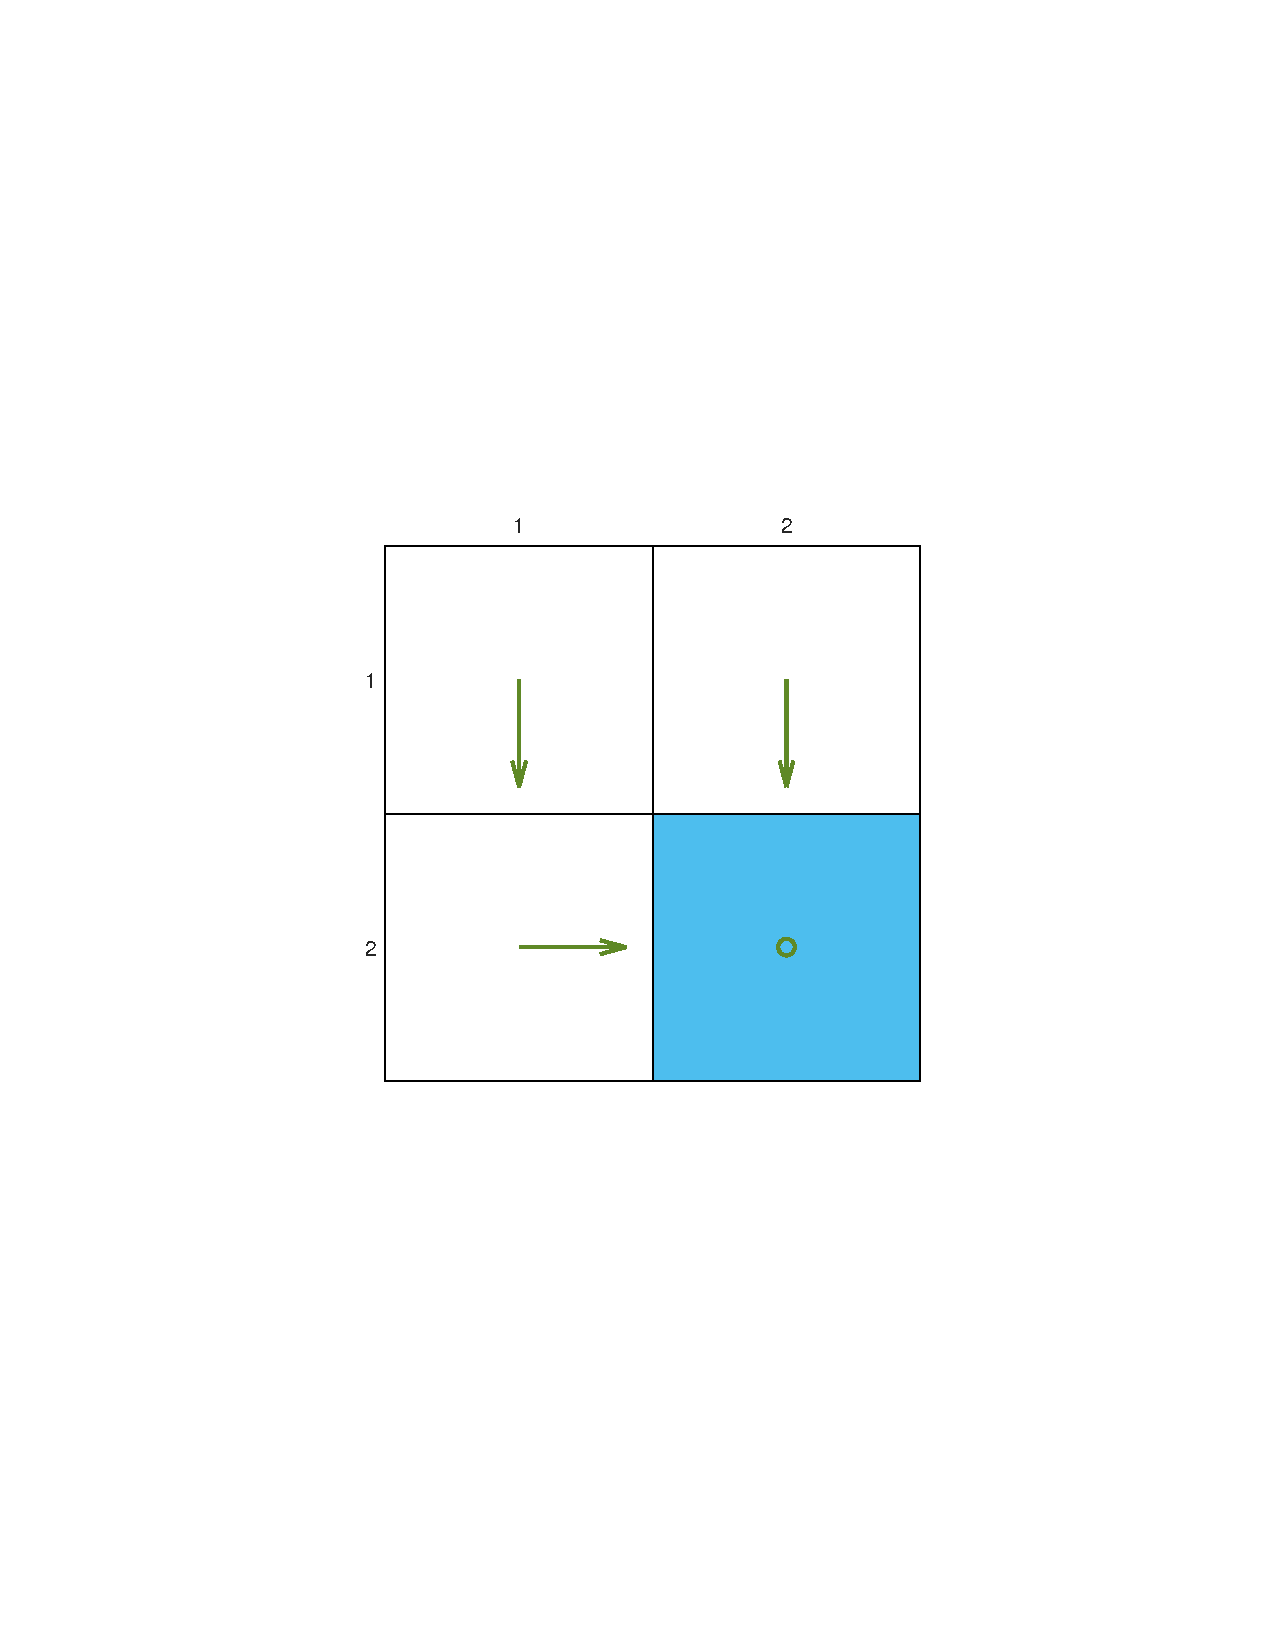
\includegraphics[width=0.2\linewidth]{fig_gridPolicy_fastest1.pdf}\,
  \includegraphics[width=0.2\linewidth]{fig_gridStateValue_fastest1}}
  \qquad\qquad
  \subfloat[Not optimal]{
  \includegraphics[width=0.2\linewidth]{fig_gridPolicy_fastest2.pdf}\,
  \includegraphics[width=0.2\linewidth]{fig_gridStateValue_fastest2}}
\end{figure}

\pause
\textbf{Question:} Why does the optimal policy not take meaningless detours? We don't punish for taking detours because $r_{\textrm{otherstep}}=0$.

\pause
\textbf{Answer:} We do punish by using the discount rate!

\pause
Policy (a):
$\rm return=1+\gamma 1+\gamma^21+\dots=1/(1-\gamma)=10$

Policy (b):
$\rm return=0+\gamma 0+\gamma^21+\gamma^31+\dots=\gamma^2/(1-\gamma)=8.1$
\end{frame}
%----------------------------------------------------
\begin{frame}
\frametitle{Summary}

Bellman optimality equation:
\begin{itemize}
\item Elementwise form:
\begin{align*}
v(s)=\blue{\max_\pi} \sum_{a}\blue{\pi(a|s)}\underbrace{\left(\sum_{r}p(r|s,a)r + \gamma \sum_{s'}p(s'|s,a)v(s')\right)}_{q(s,a)},\quad \forall s\in\mathcal{S}
\end{align*}
\vspace{-10pt}
\item
Matrix-vector form:
\vspace{-10pt}
\begin{align*}%\label{eq_bellmanOptimalityEquation_matrixForm}
\blue{v=\max_{\pi}(r_\pi+\gamma  P_\pi v)}
\end{align*}
\end{itemize}

\end{frame}
%----------------------------------------------------
\begin{frame}
\frametitle{Summary}

Questions about the Bellman optimality equation:
\begin{itemize}
\item \textbf{Existence}: does this equation have solutions?
\begin{itemize}
\item[-] \blue{Yes, by the contraction mapping theorem}
\end{itemize}
\pause
\item \textbf{Uniqueness}: is the solution to this equation unique?
\begin{itemize}
\item[-] \blue{Yes, by the contraction mapping theorem}
\end{itemize}
\pause
\item \textbf{Algorithm}: how to solve this equation?
\begin{itemize}
\item[-] \blue{Iterative algorithm suggested by the contraction mapping theorem}
\end{itemize}
\pause
\item \textbf{Optimality}: why we study this equation
\begin{itemize}
\item[-] \blue{Because its solution corresponds to the optimal state value and optimal policy.}
\end{itemize}
\end{itemize}
\pause
\textcolor{red}{Finally, we understand why it is important to study the BOE!}
\end{frame}
%%%%%%%%%%%%%%%%%%%%%%%%%%%%%%%%%%%%%%%%%%%%%%%%%%%%%%%%%%%%%%%%%%%%%%%%%%%%%%%%%%%%%%%%%%%%%%%%%%
%\bibliographystyle{plainnat}
%\bibliography{myOwnPub,zsyReferenceAll}
\end{document}
